% =====================================================================
%  NTU-DAVID-RAG — Technical report
%  Compile:  pdflatex main.tex   (run twice for refs/ToC)
%  Figures are pulled from ../drawings/ (built by drawings/build.sh)
% =====================================================================
\documentclass[11pt,a4paper]{article}

\usepackage[margin=1in]{geometry}
\usepackage{amsmath,amssymb}
\usepackage{graphicx}
\usepackage{booktabs}
\usepackage{array}
\usepackage{xcolor}
\usepackage{enumitem}
\usepackage{caption}
\usepackage{float}
\usepackage{pgfplots}
\pgfplotsset{compat=1.17}
\usepackage[colorlinks=true,linkcolor=teal!60!black,urlcolor=teal!60!black,
            citecolor=teal!60!black]{hyperref}

\graphicspath{{../drawings/}}

% ---- light section styling ----
\usepackage{titlesec}
\definecolor{accent}{RGB}{0,128,128}
\titleformat{\section}{\Large\bfseries\color{accent}}{\thesection}{0.6em}{}
\titleformat{\subsection}{\large\bfseries\color{accent!80!black}}{\thesubsection}{0.6em}{}
\captionsetup{font=small,labelfont={bf,color=accent}}

\newcommand{\code}[1]{\texttt{\small #1}}

\title{\vspace{-1.2cm}\textbf{\color{accent}NTU-DAVID-RAG}\\[2pt]
       \large A Retrieval-Augmented Generation System for\\
       Economics Research Papers and Fortran Model Code\\[6pt]
       \normalsize Technology, Pipeline, and RAGAS Evaluation}
\author{}
\date{\today}

\begin{document}
\maketitle
\vspace{-1.0cm}

\begin{abstract}
\noindent
NTU-DAVID-RAG is a retrieval-augmented generation (RAG) system that lets
researchers ask natural-language questions over a corpus of computational-economics
papers and their accompanying Fortran source code. The system pairs a structured
ingestion pipeline (PDF layout parsing, multimodal enrichment, section-aware
chunking, and dense embedding) with a hybrid retrieval pipeline (sparse BM25
$+$ dense vectors, reciprocal-rank fusion, and cross-encoder reranking) feeding a
grounded, locally hosted large language model. This report documents the
technology stack, explains the end-to-end data flow for both ingestion and
querying, describes the containerized deployment, and reports reference-free
quality measurements obtained with the RAGAS framework across several judge
models.
\end{abstract}

\tableofcontents
\vspace{0.4cm}

% =====================================================================
\section{System Overview}
% =====================================================================
The system answers two kinds of questions over a private, per-user corpus:
\emph{local} questions about a single paper (a definition, an equation, a table
value, a Fortran routine) and \emph{global} questions that compare or synthesize
across papers (``which papers use value-function iteration?''). To serve both
well it combines lexical and semantic retrieval, a paper-level profile index for
cross-document reasoning, and strict context-grounding at generation time.

The corpus is unusual for RAG in three ways that shape every design decision:

\begin{itemize}[leftmargin=1.4em,itemsep=2pt]
  \item \textbf{Heavy mathematics.} Content is dense in LaTeX equations and
        transition matrices, so extraction preserves equations and tables as
        first-class, separately describable objects.
  \item \textbf{Code alongside prose.} Each paper may ship a Fortran
        implementation; the system parses it into routine-level units with a
        call graph so questions about \code{rw\_decision} or value-function
        iteration can be answered from code, not just text.
  \item \textbf{Exact identifiers matter.} Variable and subroutine names must
        match literally, which is why a sparse BM25 stage runs alongside dense
        vectors rather than relying on embeddings alone.
\end{itemize}

% =====================================================================
\section{Technology Stack}
% =====================================================================
Table~\ref{tab:stack} summarizes the components and the role each plays in the
pipeline. The default deployment runs entirely on self-hosted infrastructure;
all model inference (embedding, reranking, generation, and the RAGAS judge) can
be served locally, with optional hosted judges used only for evaluation.

\begin{table}[H]
\centering
\small
\renewcommand{\arraystretch}{1.25}
\begin{tabular}{>{\raggedright\arraybackslash}p{3.1cm}
                >{\raggedright\arraybackslash}p{5.1cm}
                >{\raggedright\arraybackslash}p{5.6cm}}
\toprule
\textbf{Stage} & \textbf{Technology} & \textbf{Role} \\
\midrule
PDF extraction      & MinerU (GPU)                          & Convert PDF to Markdown + structured content list (text, images, equations, tables) \\
Multimodal enrich.  & Local LLM (\code{gemma4:31b} via Ollama) & Extract title/authors; describe figures, tables, and equations for indexing \\
Code digestion      & Regex parser $+$ LLM                  & Split Fortran into \code{PROGRAM/MODULE/SUBROUTINE/FUNCTION} units with a call graph \\
Chunking            & Custom, section-aware                 & 384-token chunks, 64-token overlap, hierarchical section path prepended \\
Embeddings          & \code{gte-Qwen2-7B-instruct} (3584-dim) & Asymmetric query/document vectors for dense retrieval \\
Vector store        & Qdrant (on-disk, per-user)            & Cosine search over \code{rag\_embeddings} and \code{paper\_profiles} \\
Sparse retrieval    & BM25 (\code{rank-bm25})               & Lexical match; tokenizer preserves Fortran identifiers \\
Fusion              & Reciprocal Rank Fusion ($k{=}60$)     & Merge sparse $+$ dense ranked lists \\
Reranking           & \code{bge-reranker-v2-m3} cross-encoder & Score fused candidates against the original query \\
Generation          & Local LLM (\code{gemma4:31b})         & Grounded answer with citations to paper titles \\
Serving             & Flask $+$ Gunicorn, Nginx, PostgreSQL & API, reverse proxy, auth/conversation store \\
Orchestration       & Docker Compose                        & Multi-service stack with optional single-GPU mode \\
\bottomrule
\end{tabular}
\caption{Component technology stack and the role of each stage.}
\label{tab:stack}
\end{table}

% =====================================================================
\section{End-to-End Data Flow}
% =====================================================================
Figure~\ref{fig:pipeline} shows the two halves of the system: an
\emph{ingestion} pipeline that builds the knowledge base, and a \emph{query}
pipeline that answers questions from it. The two halves meet at the Qdrant
vector database.

\begin{figure}[H]
\centering
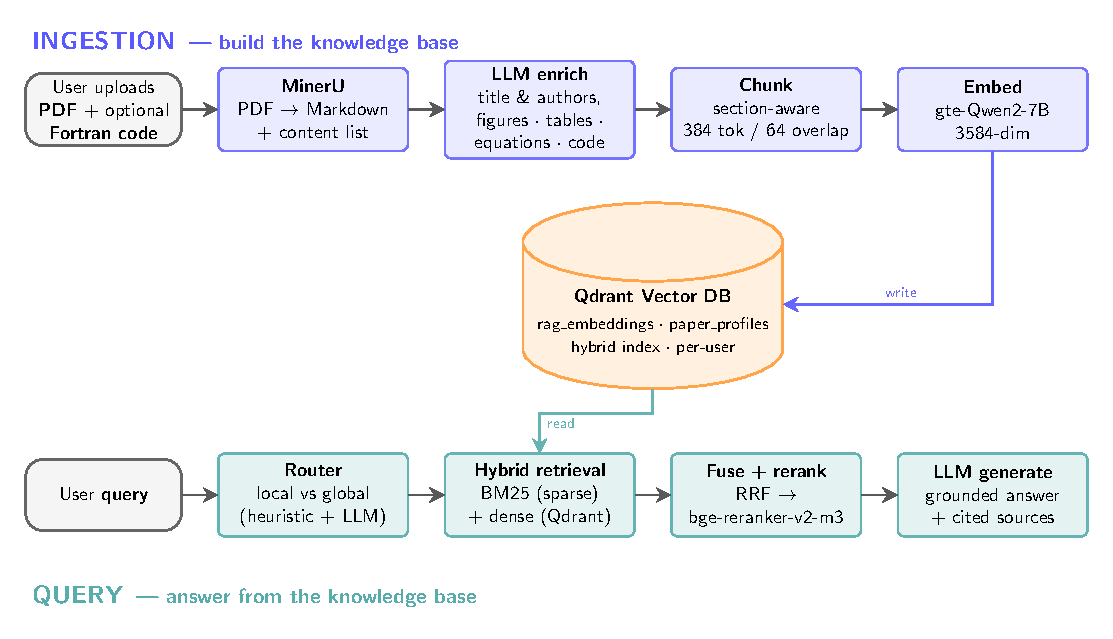
\includegraphics[width=\textwidth]{rag_pipeline.pdf}
\caption{End-to-end RAG pipeline. Ingestion (top) writes embedded, section-aware
chunks into Qdrant; querying (bottom) reads from Qdrant via hybrid retrieval,
fuses and reranks candidates, then generates a grounded answer.}
\label{fig:pipeline}
\end{figure}

\subsection{Ingestion: building the knowledge base}
A user uploads a PDF and, optionally, a Fortran source file. Ingestion proceeds
in five stages:
\begin{enumerate}[leftmargin=1.5em,itemsep=2pt]
  \item \textbf{Layout parsing (MinerU).} The PDF is converted to Markdown plus a
        \emph{content list} that tags every block as text, image, equation, or
        table, with page indices and reading order preserved.
  \item \textbf{Enrichment.} A local LLM extracts the paper title and authors and
        writes natural-language descriptions of figures, tables, and equations so
        that non-text objects become retrievable. Bibliography after
        ``References'' is stripped.
  \item \textbf{Code digestion (optional).} Fortran is parsed into routine-level
        units; each unit is summarized for its economic purpose, inputs/outputs,
        algorithm, and call relationships.
  \item \textbf{Chunking.} Manuscript text is split on section boundaries into
        384-token chunks with 64-token overlap; the hierarchical section path
        (e.g.\ \emph{IV.\ Calibration $>$ D.\ Rate of Return Process}) is
        prepended to every chunk so retrieval keeps local context. Each
        image/equation/table and each Fortran unit becomes its own document.
  \item \textbf{Embedding and indexing.} All chunks are embedded with
        \code{gte-Qwen2-7B} and upserted into Qdrant. In parallel, a per-paper
        \emph{profile} (research question, methods, key equations, concepts) is
        embedded into a separate \code{paper\_profiles} collection that powers
        global, cross-document queries.
\end{enumerate}

\subsection{Querying: answering from the knowledge base}
\begin{enumerate}[leftmargin=1.5em,itemsep=2pt]
  \item \textbf{Routing.} A heuristic-plus-LLM router classifies the query as
        \emph{local} or \emph{global} and extracts focus concepts. Global queries
        first retrieve candidate papers from the profile index, then retrieve
        within each candidate.
  \item \textbf{Hybrid retrieval.} The query is embedded for dense cosine search
        in Qdrant and, in parallel, scored by BM25. Each returns its top
        candidates.
  \item \textbf{Fusion and reranking.} The two ranked lists are merged with
        Reciprocal Rank Fusion ($k{=}60$); the fused set is reranked by the
        \code{bge-reranker-v2-m3} cross-encoder against the \emph{original} user
        query, and paper-diversity is enforced so results are not dominated by a
        single document.
  \item \textbf{Context assembly and generation.} The top passages are assembled
        into a structured context (grouped by paper, with equations/tables/code
        rendered appropriately) and passed to the generation LLM, which is
        instructed to answer only from the supplied context and cite papers by
        title. Conversation history is compacted when the prompt would exceed the
        context budget.
\end{enumerate}

% =====================================================================
\section{Deployment Architecture}
% =====================================================================
The system ships as a Docker Compose stack (Figure~\ref{fig:deploy}). A public
Nginx reverse proxy fronts the \code{rag-web} Flask application, which
orchestrates ingestion and querying. GPU-bound model inference is isolated in a
dedicated \code{embedding-server} (embeddings $+$ reranking) and an Ollama LLM
service; PostgreSQL stores users, sessions, and conversations; and each user
gets an isolated on-disk Qdrant collection set. A single-GPU override swaps in a
smaller embedder (\code{embeddinggemma-300m}) and an in-stack quantized LLM so
the whole stack fits on one card.

\begin{figure}[H]
\centering
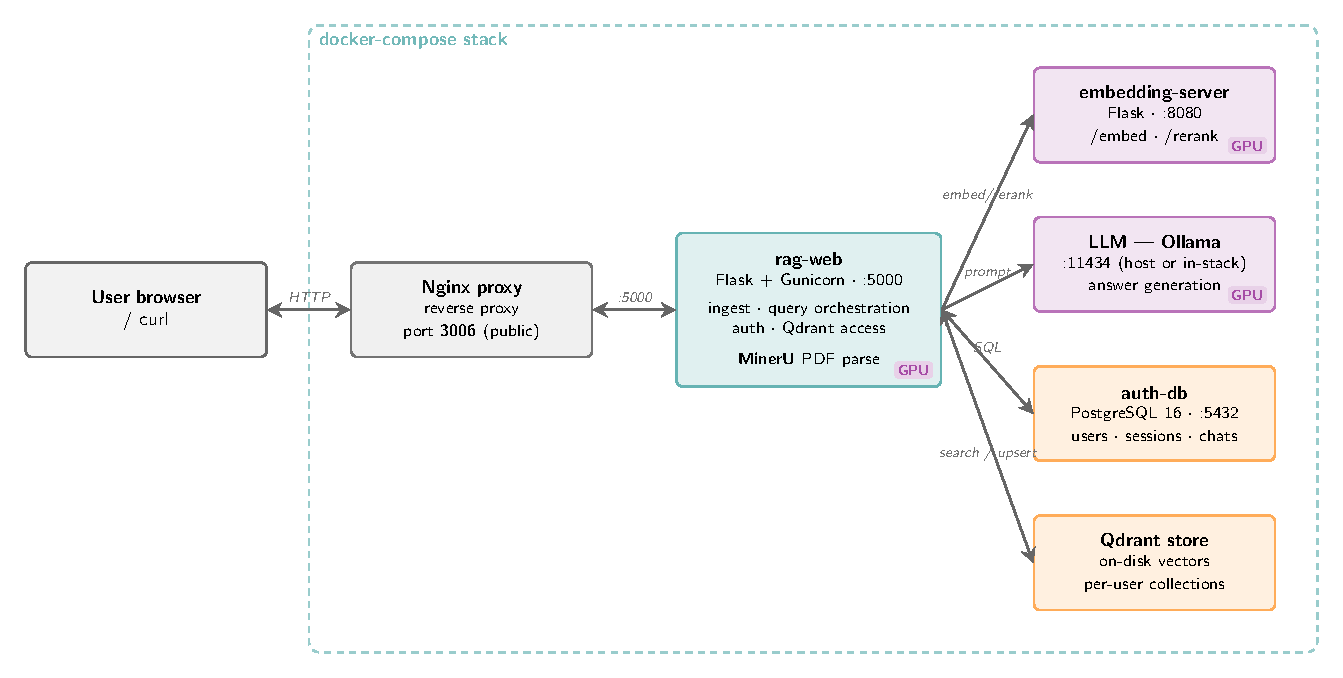
\includegraphics[width=0.95\textwidth]{rag_deployment.pdf}
\caption{Containerized service topology. \code{rag-web} is the orchestration hub;
GPU services (badged) handle embedding/reranking, PDF parsing, and generation;
PostgreSQL and per-user Qdrant provide durable state.}
\label{fig:deploy}
\end{figure}

% =====================================================================
\section{Evaluation Methodology (RAGAS)}
% =====================================================================
Quality is measured with \href{https://docs.ragas.io}{RAGAS}, a
\emph{reference-free} evaluation framework: it scores answers without
gold-standard references by using an LLM judge to inspect the question, the
generated answer, and the retrieved contexts. Two metrics are reported:

\begin{itemize}[leftmargin=1.4em,itemsep=2pt]
  \item \textbf{Faithfulness} — the fraction of claims in the answer that are
        directly supported by the retrieved context. It penalizes any statement
        the context does not entail (a proxy for hallucination).
  \item \textbf{Context Precision (without reference)} — whether the retrieved
        passages that were used are actually relevant to the question, i.e.\ the
        signal-to-noise ratio of retrieval as judged by the LLM.
\end{itemize}

The evaluation harness (\code{RAG\_quality\_test/rag\_ragas\_eval.py}) issues a
fixed question set against the live RAG API, captures each answer together with
its retrieved contexts, and scores every item with a configurable judge
(\emph{local} Ollama, \emph{OpenAI}, or \emph{Gemini}). The question set is
designed so that each item stresses a distinct facet of the pipeline:
single-paper factual and methodology retrieval, cross-paper comparative
reasoning (the global/profile path), Fortran code retrieval, LaTeX equation
retrieval, table/numeric retrieval, and an out-of-scope robustness probe whose
correct answer is ``none of the papers.''

% =====================================================================
\section{Results}
% =====================================================================
Table~\ref{tab:runs} summarizes five evaluation runs that vary the judge model,
question-set size, and \code{top\_k}. The corpus contained 5--6 papers depending
on the run.

\begin{table}[H]
\centering
\small
\renewcommand{\arraystretch}{1.2}
\begin{tabular}{l c l c c c}
\toprule
\textbf{Date} & \textbf{\#Q} & \textbf{Judge model} & \textbf{top\_k}
  & \textbf{Faithfulness} & \textbf{Context Prec.} \\
\midrule
2026-04-18 & 1  & openai / gpt-5.4              & 10 & 0.333 & 0.700 \\
2026-04-18 & 30 & gemini / gemini-2.5-flash     & 10 & \textbf{0.220} & \textbf{0.344} \\
2026-04-18 & 30 & openai / gpt-4o-2024-08-06    & 10 & 0.216 & 0.289 \\
2026-04-20 & 30 & local / gemma4:31b           & 10 & 0.125 & 0.308 \\
2026-05-12 & 10 & local / gemma4:31b           &  5 & 0.235 & 0.267 \\
\bottomrule
\end{tabular}
\caption{RAGAS aggregate means across runs. The single-question run is a smoke
test. The two hosted judges (Gemini, GPT-4o) agree closely on faithfulness
($\approx 0.22$); the local judge is harsher and far slower.}
\label{tab:runs}
\end{table}

\paragraph{Headline run.} The most representative run is the 30-question,
Gemini-judged evaluation (\code{top\_k}=10). Its per-question scores are shown in
Figure~\ref{fig:perq}. Mean faithfulness is $0.220$ (median $0.218$) and mean
context precision is $0.344$ (median $0.000$). Per-question latency averaged
$82.8$\,s (median $75.2$\,s, range $43$--$172$\,s), reflecting the cost of local
generation over long, math-heavy contexts.

\begin{figure}[H]
\centering
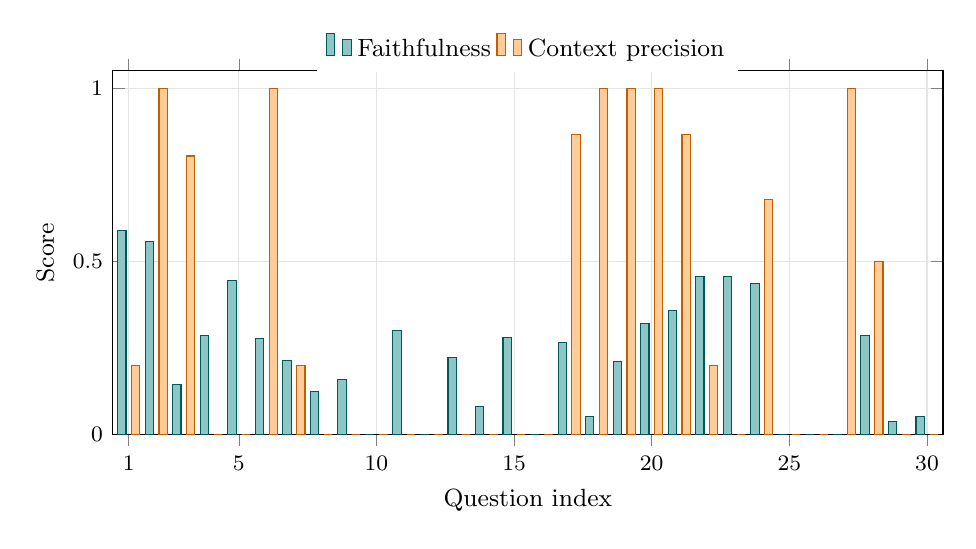
\begin{tikzpicture}
\begin{axis}[
    width=\textwidth, height=6.2cm,
    ybar, bar width=3pt,
    ymin=0, ymax=1.05,
    enlarge x limits=0.02,
    xtick={1,5,10,15,20,25,30},
    xlabel={Question index}, ylabel={Score},
    legend style={at={(0.5,1.12)},anchor=north,legend columns=2,draw=none,font=\small},
    tick label style={font=\footnotesize},
    label style={font=\small},
    grid=major, grid style={black!10},
]
\addplot[draw=teal!70!black,fill=teal!45] coordinates {
(1,0.588)(2,0.556)(3,0.143)(4,0.286)(5,0.444)(6,0.276)(7,0.214)(8,0.125)(9,0.158)(10,0.0)
(11,0.3)(12,0.0)(13,0.222)(14,0.08)(15,0.28)(16,0.0)(17,0.265)(18,0.053)(19,0.211)(20,0.321)
(21,0.357)(22,0.455)(23,0.455)(24,0.435)(25,0.0)(26,0.0)(27,0.0)(28,0.286)(29,0.038)(30,0.051)};
\addplot[draw=orange!75!black,fill=orange!40] coordinates {
(1,0.2)(2,1.0)(3,0.804)(4,0.0)(5,0.0)(6,1.0)(7,0.2)(8,0.0)(9,0.0)(10,0.0)
(11,0.0)(12,0.0)(13,0.0)(14,0.0)(15,0.0)(16,0.0)(17,0.867)(18,1.0)(19,1.0)(20,1.0)
(21,0.867)(22,0.2)(23,0.0)(24,0.679)(25,0.0)(26,0.0)(27,1.0)(28,0.5)(29,0.0)(30,0.0)};
\legend{Faithfulness, Context precision}
\end{axis}
\end{tikzpicture}
\caption{Per-question RAGAS scores for the 30-question Gemini-judged run.
Context precision is strongly bimodal: 9/30 questions score $\ge 0.8$ while
16/30 score $0$ — retrieval is either on-target or off-target, rarely in
between.}
\label{fig:perq}
\end{figure}

\subsection{Interpretation}
\begin{itemize}[leftmargin=1.4em,itemsep=3pt]
  \item \textbf{Faithfulness scores are conservative by construction.} RAGAS
        decomposes an answer into atomic claims and requires each to be entailed
        by the retrieved context. Answers in this domain are dense with LaTeX,
        matrices, and derived statements; a judge that cannot verify a transcribed
        equation token-for-token marks the claim unsupported, deflating the score.
        The close agreement between two independent hosted judges
        ($0.220$ vs.\ $0.216$) indicates the \emph{ranking} is stable even if the
        absolute level is pessimistic.
  \item \textbf{Context precision is bimodal} (Figure~\ref{fig:perq}): retrieval
        tends to either surface the right passages or miss them, with little
        middle ground. The misses cluster on equation/table/numeric questions,
        where the answer hinges on one specific block that must be retrieved
        verbatim — the motivation for the hybrid BM25 stage and the multimodal
        equation/table indexing.
  \item \textbf{Judge choice matters.} The local \code{gemma4:31b} judge is both
        harsher on faithfulness ($0.125$) and dramatically slower (264 minutes for
        30 questions vs.\ ${\sim}53$--$71$ minutes for hosted judges), making it
        useful for offline regression but unsuitable for fast iteration.
  \item \textbf{Latency is generation-bound.} End-to-end time is dominated by
        local LLM generation over long contexts, not by retrieval; longer answers
        (equation/derivation questions) sit at the high end of the latency range.
\end{itemize}

\subsection{Two-GPU vs.\ single-GPU deployment (per-question)}
To quantify what single-GPU mode costs (or gains), the same 10-question set was
run against both deployments with the generator, judge, and \code{top\_k} held
fixed (\code{gemma4:31b} generation, local \code{gemma4:31b} judge,
\code{top\_k}=5). The only differences are the GPU count and the embedder: the
default two-GPU stack runs the 7B \code{gte-Qwen2-7B} embedder (3584-dim) on a
separate card from the generator, while the single-GPU stack collapses every
component onto one card with the lighter \code{bge-large-en-v1.5} embedder
(1024-dim).\footnote{The single-GPU override's default embedder,
\code{embeddinggemma-300m}, is gated on Hugging Face; the evaluated run
substituted the non-gated \code{bge-large-en-v1.5}.} The comparison therefore
isolates the effect of moving to a single card.

Table~\ref{tab:2v1} reports the per-question scores and their difference
($\Delta = \text{single-GPU} - \text{two-GPU}$); Figure~\ref{fig:2v1delta}
visualizes the same deltas.

\begin{table}[H]
\centering
\small
\renewcommand{\arraystretch}{1.15}
\begin{tabular}{c l cc cc cc}
\toprule
& & \multicolumn{2}{c}{\textbf{2-GPU (gte-Qwen)}}
  & \multicolumn{2}{c}{\textbf{1-GPU (bge-large)}}
  & \multicolumn{2}{c}{\textbf{Difference}} \\
\cmidrule(lr){3-4}\cmidrule(lr){5-6}\cmidrule(lr){7-8}
\textbf{Q} & \textbf{Facet} & F & CP & F & CP & $\Delta$F & $\Delta$CP \\
\midrule
1  & single-paper factual      & 0.13 & 0.00 & 0.38 & 1.00 & $+0.25$ & $+1.00$ \\
2  & single-paper factual      & 0.67 & 0.00 & 0.36 & 0.33 & $-0.30$ & $+0.33$ \\
3  & methodology               & 0.06 & 1.00 & 0.88 & 1.00 & $+0.82$ & $0.00$  \\
4  & cross-paper comparative   & 0.00 & 0.00 & 0.30 & 0.00 & $+0.30$ & $0.00$  \\
5  & cross-paper comparative   & 0.00 & 0.00 & 0.00 & 0.00 & $0.00$  & $0.00$  \\
6  & cross-paper comparative   & 0.00 & 0.00 & 0.00 & 0.00 & $0.00$  & $0.00$  \\
7  & Fortran / code            & 1.00 & 0.83 & 0.36 & 1.00 & $-0.64$ & $+0.17$ \\
8  & equation / formula        & 0.50 & 0.00 & 0.71 & 1.00 & $+0.21$ & $+1.00$ \\
9  & table / numeric           & 0.00 & 0.83 & 0.00 & 0.00 & $0.00$  & $-0.83$ \\
10 & robustness (out-of-scope) & 0.00 & 0.00 & 0.00 & 0.00 & $0.00$  & $0.00$  \\
\midrule
\multicolumn{2}{l}{\textbf{Mean}} & 0.235 & 0.267 & 0.299 & 0.433
  & $\mathbf{+0.064}$ & $\mathbf{+0.166}$ \\
\bottomrule
\end{tabular}
\caption{Per-question RAGAS scores for the two-GPU and single-GPU deployments
(F~=~faithfulness, CP~=~context precision) with the single-GPU\,$-$\,two-GPU
difference. Generator, judge, question set, and \code{top\_k} are identical; only
the embedder and GPU count differ. The single-GPU stack improves both means.}
\label{tab:2v1}
\end{table}

\begin{figure}[H]
\centering
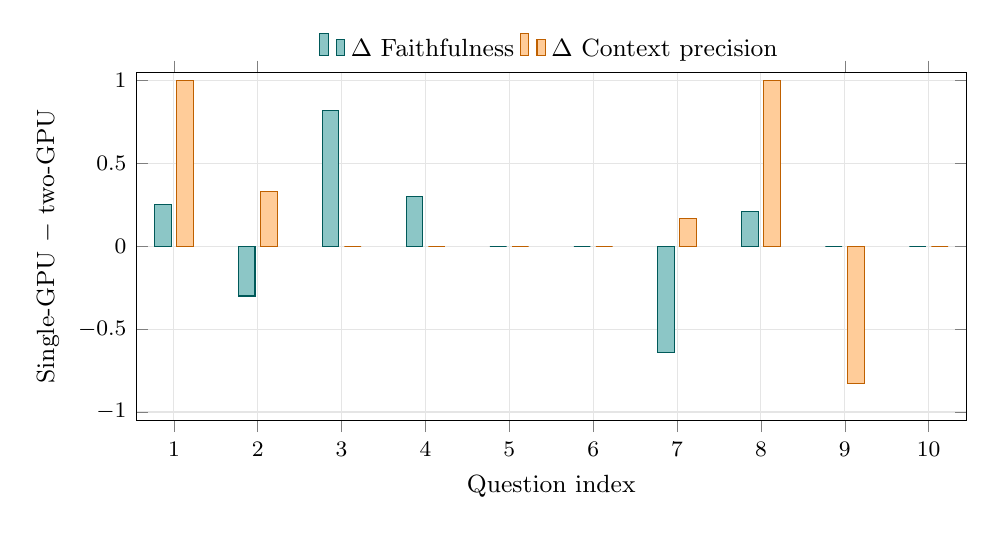
\begin{tikzpicture}
\begin{axis}[
    width=\textwidth, height=6.0cm,
    ybar, bar width=6pt,
    ymin=-1.05, ymax=1.05,
    enlarge x limits=0.05,
    xtick={1,2,3,4,5,6,7,8,9,10},
    xlabel={Question index}, ylabel={Single-GPU $-$ two-GPU},
    legend style={at={(0.5,1.13)},anchor=north,legend columns=2,draw=none,font=\small},
    tick label style={font=\footnotesize},
    label style={font=\small},
    grid=major, grid style={black!10},
]
\addplot[draw=teal!70!black,fill=teal!45] coordinates {
(1,0.25)(2,-0.30)(3,0.82)(4,0.30)(5,0)(6,0)(7,-0.64)(8,0.21)(9,0)(10,0)};
\addplot[draw=orange!75!black,fill=orange!40] coordinates {
(1,1.0)(2,0.33)(3,0)(4,0)(5,0)(6,0)(7,0.17)(8,1.0)(9,-0.83)(10,0)};
\legend{$\Delta$ Faithfulness, $\Delta$ Context precision}
\end{axis}
\end{tikzpicture}
\caption{Per-question change from the two-GPU to the single-GPU deployment
(positive $=$ single-GPU better). Both means rise; gains concentrate on factual
and equation retrieval (Q1, Q8, which jump from $0$ to $1.0$ context precision),
while the two regressions are exact-identifier retrieval (Q7, the Fortran
\code{rw\_decision} routine) and exact-table retrieval (Q9).}
\label{fig:2v1delta}
\end{figure}

\paragraph{Interpretation.} Counter-intuitively, collapsing onto a single GPU
\emph{improves} both aggregate metrics ($+0.064$ faithfulness, $+0.166$ context
precision). The gain is driven by the embedder: \code{bge-large} surfaces the
relevant passage on factual and equation questions where the larger
\code{gte-Qwen} embedder missed (Q1 and Q8 move from $0$ to perfect context
precision). The two regressions are both exact-block retrieval --- the
code-pretrained \code{gte-Qwen} ranked the precise Fortran routine into the top
contexts (Q7) and retrieved the target table (Q9), whereas the prose-oriented
\code{bge-large} did not --- reinforcing exact identifier/table retrieval as the
highest-value improvement target. Cross-paper comparison (Q5--Q6) and the
out-of-scope probe (Q10) score zero on \emph{both} deployments, confirming these
are pipeline-level gaps independent of the embedder or GPU budget. For reference,
a single-GPU run with the lighter \code{gemma3:12b-int4} generator in place of
\code{gemma4:31b} reached the same context precision ($0.450$) at lower
faithfulness ($0.216$), indicating that the embedder governs retrieval precision
while the generator governs faithfulness.

\subsection{Threats to validity}
These are reference-free, LLM-judged measurements on a small (10--30 question)
set over a 5--6 paper corpus, so absolute values should be read as relative
signals rather than benchmarks. Faithfulness in particular under-credits
correct-but-hard-to-verify mathematical content. The intended use is regression
tracking and \emph{controlled} A/B comparisons --- such as the two-GPU vs.\
single-GPU study above, which fixes the judge, question set, generator, and
\code{top\_k} so that only the deployment varies --- rather than absolute
cross-benchmark claims.

% =====================================================================
\section{Conclusion}
% =====================================================================
NTU-DAVID-RAG combines structure-aware ingestion (layout parsing, multimodal
enrichment, code digestion, section-aware chunking) with a hybrid retrieval stack
(BM25 $+$ dense $+$ RRF $+$ cross-encoder reranking) and a grounded local LLM,
all deployed as an isolated, per-user Docker stack. RAGAS evaluation shows stable,
judge-agnostic faithfulness around $0.22$ and a bimodal context-precision profile
that pinpoints equation/table retrieval as the highest-value target for further
work — improving exact-block retrieval for mathematical content is expected to
lift both metrics simultaneously.

\end{document}
